\part{Explorations}
\chapter{Trois Cas Observes}

\paragraph{} Le XXIe siècle et ses innombrables moyens de communication ont
rendu les situations interculturelles de plus en plus courantes. C'est pourquoi
le choc des cultures est une expérience que chaque Français est amené à vivre
quotidiennement. Cette expérience peut émerveiller, interpeller ou choquer
comme vu ci-dessous.

\section{Émerveillement}

\subsection{1\iere version}

\paragraph{} En France peu de tradition ont perduré au cours du temps. En
effet, la France étant un pays issue de nombreux brassage, les habitudes et les
traditions sont propres à chaque famille. Au contraire, le Japon, bien qu'étant
très avancé au niveau des nouvelles technologies, a su garder nombre de ses
traditions tel que le fait d'aller au temple prier pour la nouvelle année. Cela
m'étonne toujours avec plaisir de penser à ce contraste qui cohabite entre la
culture traditionnelle et la culture moderne japonaise.

\subsection{2\ieme version}

\begin{center}
	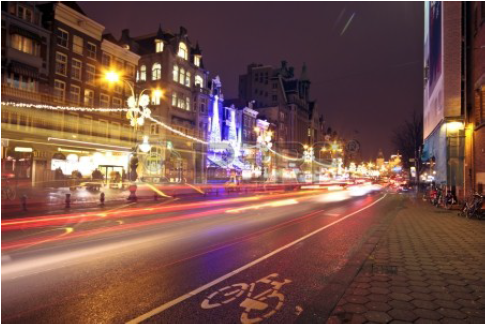
\includegraphics[scale=0.7]{Amsterdam1.jpg}
\end{center}

\paragraph{} Parmi les situations qui m'a le plus émerveillé, c'est bien le
jour où j'ai vu deux sans abris aux alentours d'Amsterdam.  Nous étions la
veille de noël et j'ai vu ces deux personnes par terre se raconter des
histoires et rigoler ensemble. Cette scène m'a paru inespérée car il faisait
froid, mais ils avaient l'air si heureux.  Cette scène m'a fait rendre compte
que nous devons profiter de chaque moment de notre vie et que dans toutes les
situations, nous devons savoir rire et être heureux.

\begin{center}
	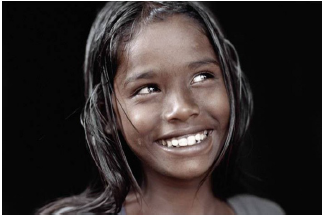
\includegraphics[scale=0.7]{Amsterdam2.jpg}
\end{center}

\paragraph{} De nos jours, de grandes inégalités sociales ont vues le jour et
nous devons les combattre pour que personne ne meurt de froid ou de faim. Je me
rends compte que le bonheur ne vient pas seul, il faut porter de l'attention à
quiconque, car nous partageons cette même planète.  Cette expérience de vie m'a
fait comprendre beaucoup sur l'homme et sur ce dont il a besoin. Nous devons
être heureux ensemble, apprenons à vivre tous ensemble en s'entraidant.

\subsection{3\ieme version}

\paragraph{} Des contacts interculturels qui m'ont émerveillés et qui
continuent encore de m'émerveiller sont le fait que les différences culturelles
sur internet dans le domaine de l'informatique sont complètement ignorées. En
effet, lorsque le sujet est différent de l'interculturalité les personnes sur
internet parlent en général librement sans prendre considération de l'origine
ou de la culture de l'autre. J'en conclue donc que de par le fait qu'ils
n'aient pas de contacts visuels directs avec les personnes, ils ne
réfléchissent pas à l'origine ou à la culture de l'autre, ce qui m'incline à
penser que le principal facteur des dissonances interculturelles est le contact
visuel.

\subsection{4\ieme version}

\paragraph{} Ayant peu voyagé, je n'ai pas pu connaître beaucoup de situations
interculturelles fortes. Cependant, un exemple récent me vient en tête. J'ai
suivi à la télévision et sur Internet les images des manifestations pour la
paix du 11 janvier 2015 à Paris et dans les grandes villes françaises. Alors
que le clivage entre les cultures me semblait se développer dans notre pays, et
que le ``creuset français'' (Gérard Noiriel) ne semblait plus une réalité,
cette manifestation m'a montré qu'une France hétérogène – dans ses origines –
mais uniforme – dans ses idéaux – existait toujours. Certes, nombreux étaient
ceux qui ont participé à ces marches pour prouver ou revendiquer une position,
comme les nombreux chefs d'État présents, ou les représentants religieux venus
dénouer les ambiguïtés entre religion et obscurantisme. Cependant, l'image
d'une foule issue de toutes les cultures et toutes les religions arborant les
couleurs françaises ou même celles de Charlie Hebdo, un journal plutôt connu
pour diviser que rassembler, était un symbole fort. Des banderoles de la
citation attribuée à Voltaire par une biographe anglaise s'étalaient en
plusieurs langues: ``I disapprove of what you say, but I will defend to the
death your right to say it''. Cela peut sembler mièvre et patriotique, mais il
semblait se dégager un ``esprit français''.

\begin{center}
	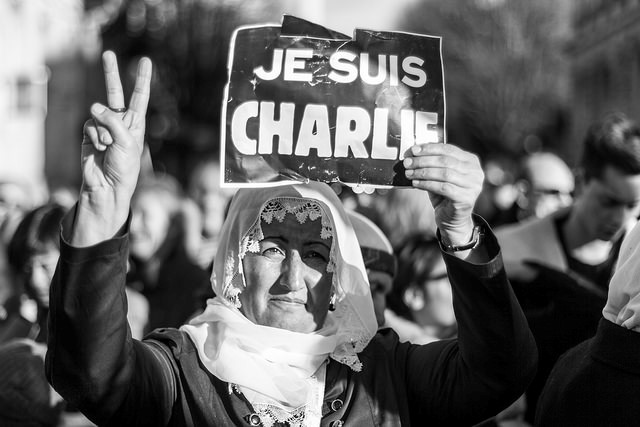
\includegraphics[scale=0.5]{charlie.jpg}
\end{center}

\section{Interpellation}
\subsection{1\iere version}

\paragraph{} J'ai participé à trois voyages scolaires durant mes années de
lycée.  Lors des voyages en Irlande du Nord et en Angleterre, nous avons
séjourné dans des familles d'accueil. Lors du voyage en Angleterre, je n'ai pu
apercevoir qu'une seule fois le mari et les enfants. En effet, seule la
maitresse de maison s'occupait de nous et nous accordait du temps. Cependant,
bien qu'elle fût accueillante, nous prenions nos repas entre nous sans la
famille. C'est ainsi que nous avons passé ces quelques jours dans cette famille
sans beaucoup de contact avec celle-ci. Au contraire, lors du voyage en
Irlande, nous prenions tous nos repas avec les parents de la famille. En effet,
les enfants ayant un rythme de vie moins souple mangeaient aux heures
habituelles pour leur culture tandis que les parents nous attendaient pour
manger avec nous lorsque nous rentrions le soir. Cependant, nous avons pu voir
certain des enfants le soir qui venaient discuter avec nous et les parents
pendant qu'on prenait notre repas et eux se contentaient d'un thé. Ainsi, nous
avons pu discuter des différences de culture entre les Irlandais et les
étudiants qu'ils accueillaient, de leur histoire (ce pourquoi nous faisions ce
voyage scolaire), etc\ldots Je fus donc interpellé par la différence d'accueil
entre les Anglais et les Irlandais. Bien que chacune des familles étaient payée
par une association pour nous accueillir, le ressenti ne fut pas le même: les
Irlandais nous accueillait aussi par envie et pas seulement pour l'argent.

\subsection{2\ieme version}

\begin{center}
	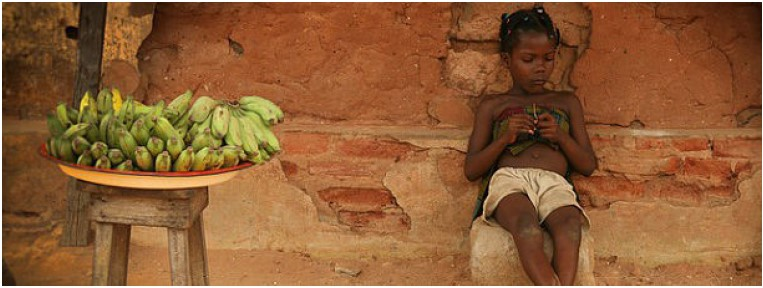
\includegraphics[scale=0.7]{Afrique.jpg}
\end{center}

\paragraph{} Ce qui m'a émerveillé, c'est de voir ma cousine partir en Afrique,
plus précisément au Liberia, pour combattre une maladie qui a fait énormément
de mort, appelé Ébola.  Travaillant dans l'humanitaire, elle m'a toujours
passionné par tout ce qu'elle a accomplie jusqu'à présent. Ces derniers temps,
j'ai été fasciné par son courage d'entreprendre les choses et son désir de
vouloir aider ces personnes, souffrant de l'Ébola.

\begin{center}
	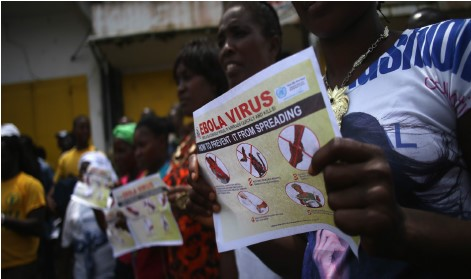
\includegraphics[scale=0.7]{Afrique2.jpg}
\end{center}

\paragraph{} Actuellement, elle est une des managers d'une ONG en santé
publique, permettant de limiter la contamination du virus. Elle me raconte par
mails ses journées et comment est-ce qu'elle fait pour ne pas craquer
émotionnellement. Ses différentes expériences à travers le monde m'ont donné
l'envie de voyager et d'aider les personnes qui m'entourent.

\subsection{3\ieme version}

\paragraph{} Ce qui m'a interpellé lors d'un voyage en Allemagne est le fait
que les allemands mangent de la charcuterie au petit déjeuner. Après des études
approfondies, j'ai jugé que ce rituel culturel méritait sa place en Allemagne
et sûrement dans d'autres pays. C'est du moins ce que mes papilles gustatives
en ont déduit.

\subsection{4\ieme version}

\paragraph{} Il y a près de quatre ans, je suis parti en Angleterre pendant
deux semaines avec un ami. Ses parents l'avaient poussé à partir pour un séjour
linguistique en groupe, et je l'ai accompagné. Je me suis donc retrouvé avec
lui en famille d'accueil, et je pensais que nous serions souvent en contact
avec les ``natifs''. J'ai assez vite déchanté: les familles d'accueil sont une
industrie anglaise! Dans cette petite maison, nous étions quatre étrangers
d'origines différentes, mais la famille habituée ne jouait pas la carte du
melting-pot: nous étions dans des chambres différentes, nous n'étions pas
soumis aux mêmes horaires, nous avions rempli un formulaire sur les plats que
nous n'aimions pas\ldots De même, lors des sorties organisées par le groupe, et
lors des cours d'anglais organisés par un professeur non francophone, les
jeunes français (qui pourtant ne se connaissaient pas) s'isolaient pour
discuter entre eux. Cela peut sembler naturel: timidité, hésitation à parler en
anglais\ldots Mais les organisateurs ne faisaient rien contre, que ce soient
les Français tout aussi hésitants ou les Anglais habitués à ce genre de
situation. Finalement, je n'ai pas progressé en anglais au cours de ce voyage,
et n'ai connu aucune situation interculturelle. Bien que timide de nature, j'en
étais très déçu.

\section{Choc}

\subsection{1\iere version}

\paragraph{} Un été je suis partie une semaine en Toscane. Ne pouvant pas
marcher longtemps suite à de nombreuses entorses, nous avons fait le tour de la
Toscane en voiture en nous arrêtant dans les villes plus ou moins touristique
sur notre chemin (Florence, Pise, etc\ldots).  En arrivant sur Florence, nous avons
pris une route à deux voies. Nous avons vu devant nous trois voitures côtes à
côtes.  Cela m'a choqué de voir ce manque de respect pour le code de la route
et ce mépris du danger. En effet, les Français ne sont pas toujours les
meilleurs dans le respect du code de la route mais ça n'en devient pas un sport
national comme en Italie: nous avons vu de nombreuses absences de respect du
code de la route.

\subsection{2\ieme version}

\begin{center}
	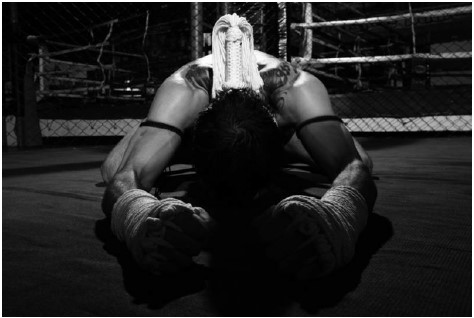
\includegraphics[scale=0.7]{Thai1.jpg}
\end{center}

\paragraph{} Lors d'un voyage à Thaïlande, j'ai décidé de découvrir la boxe
thaïlandaise, appelé plus communément ``Muay Thai'' dans le pays de provenance
de cet art martial. La boxe thaïlandaise se base sur quatre techniques
fondamentales: les coups de poings, pieds, genoux et coudes. Les boxeurs
portent des gants et un short afin de faciliter les mouvements des jambes. Les
combats s'effectuent en 5 reprises de 3 minutes entrecoupées de pause de 2
minutes. Le tout se déroule sur une musique de fond thaïlandaise très
envoutante.  Quelques jours après mon arrivée, je me baladais dans les rues du
quartier de Sukhumvit, dans des avenues très vivantes, jours et nuits sur toute
leur longueur, je me suis dirigé vers un bâtiment qui ressemblait à un temple.
Tout le monde criait et voulait y rentrer, j'ai convaincu les amis avec qui
j'étais d'y aller, pour voir de quoi est-ce qu'il s'agissait.  L'entrée était
gratuite, mais il y avait des guichets où nous pouvions miser de l'argent sur
des numéros. Ces numéros étaient tout simplement des boxeurs et nous étions
arrivés en face d'un ring de boxe autour duquel se trouvait une foule
incroyable.

\begin{center}
	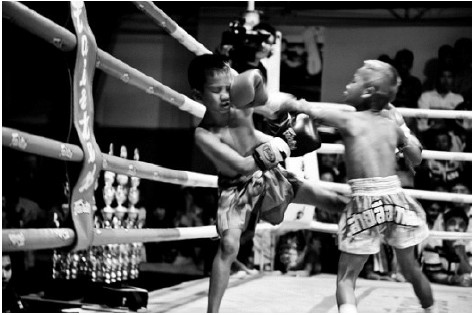
\includegraphics[scale=0.7]{Thai2.jpg}
\end{center}

\paragraph{} Sur le ring, se trouvait deux enfants âgés de 8 ans combattant
l'un contre l'autre sous les applaudissements et les encouragements d'adultes
qui criait victoire pour la personne sur laquelle il avait misé. Cette scène
eut l'effet d'un tonnerre qui s'abattit sur moi, car je ne pouvais rien à faire
pour arrêter ce massacre.  Malheureusement, j'ai demandé aux spectateurs la
raison pour laquelle ils se battaient et on me répondit ``de baht!'', qui veut
dire ``pour l'argent'' en thaïlandais. Totalement outragé de voir ce qu'il se
passait en Thaïlande, j'ai décidé de retrouver le jeune boxeur ayant perdu et
n'ayant pas gagné d'argent, pour le féliciter et lui donner 400 bahts, qui est
l'équivalent de 10 euros, mais qui représente une somme énorme pour eux.  Ces
découvertes m'ont mis totalement mal à l'aise et j'ai décidé de combattre cette
cause en revenant à la source, la pauvreté.

\begin{center}
	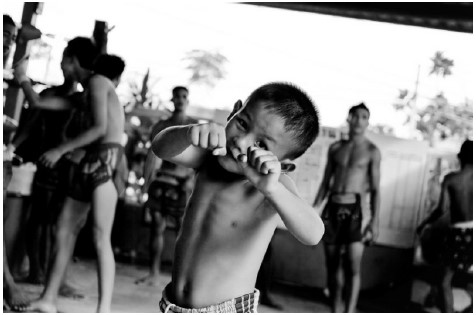
\includegraphics[scale=0.7]{Thai3.jpg}
\end{center}

\subsection{3\ieme version}

\paragraph{} Une situation qui m'a choqué en étant en voyage au Sri-Lanka est
la conduite de ces derniers. En effet, il m'est arrivé d'être à quatre voitures
sur une route à deux voies à sens alternés. J'en ai donc déduit que les
Sri-Lankais se faisaient confiance au point d'avoir ce genre d'``interactions''
sur la route.

\subsection{4\ieme version}

\paragraph{} Ma famille est très attachée au patrimoine: mon père et ma mère
sont des spécialistes des monuments historiques, mon grand-père et mon oncle
sont antiquaires. J'ai donc été élevé dans cette ambiance, ne partant en voyage
que pour visiter des églises. C'est pourquoi, lors d'un séjour à Venise où,
étant très jeune, je ne prêtais pas grande attention à la culture locale, j'ai
été frappé par l'approche différente que l'Italie a de la culture. En effet, de
nombreuses églises, du fait du nombre de touristes, font payer les visiteurs à
l'entrée! Cela me semblait inconcevable, d'autant que je n'étais pas certain
que cet argent irait à la paroisse! Plus tard, lors d'un voyage scolaire à
Pompéi, j'ai remarqué l'état de délabrement de la cité millénaire, qui est dû à
l'absence de moyens de conservation plus qu'aux dégâts infligés par le Vésuve.
Plusieurs bâtisses se sont effondrées, redressées à la va-vite avec du béton et
cachées à la vue des visiteurs par des pancartes. Un bâtiment du forum a même
été transformé en cafétéria. Ma mère m'expliqua que l'argent des visiteurs
n'allait pas à la conservation du site mais plus ou moins à la pègre locale
(n'oublions pas qu'il s'agit de Naples!). Si l'Italie comme la France jouit
d'un patrimoine exceptionnel, l'approche italienne est beaucoup plus
économique! J'en étais d'autant plus attristé qu'avec Pompéi peut disparaître
une portion d'histoire.

\begin{center}
	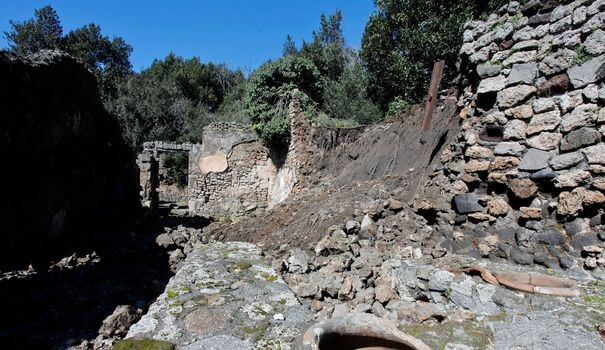
\includegraphics[scale=0.5]{Pompei.jpg}
\end{center}

\chapter{Bienvenue au café}

\paragraph{} Chaque café possède sa propre vie, sa propre ambiance qui varie
suivant l'heure, le jour et leur voisinage. Du café de la gare peuplée de
voyageurs au comptoir montagnard abritant les skieurs frigorifiés, en faisant
un détour par Londres, nous allons vous donner un aperçu de l'atmosphère
typique de ces lieux de rencontres.

\section{1\iere version}

\paragraph{} La vie des cafés varie grandement suivant leur situation
géographique, la météo et la période.

\paragraph{} Prenons deux cafés dans une même station de ski familiale dans le
massif central: la brasserie des pistes, vu entre 18h45 et 19h30, fait
bar/brasserie/restaurant ; le polar beer, vu entre 16h et 17h, fait bar toute
la journée et snack le midi. Il se situe juste en bas des pistes.

\begin{center}
	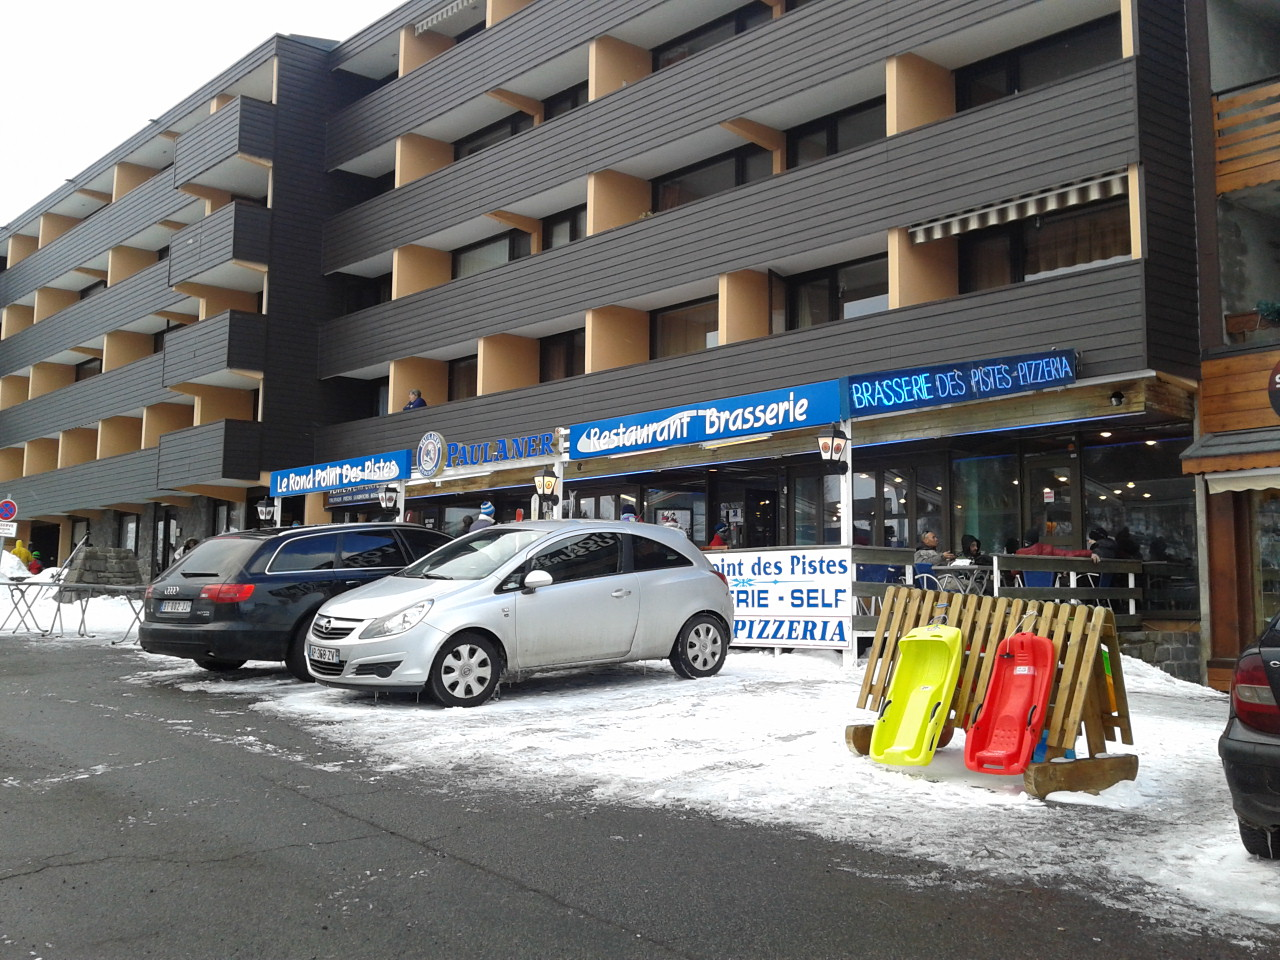
\includegraphics[scale=0.15]{brasserieDesPistes.jpg}
	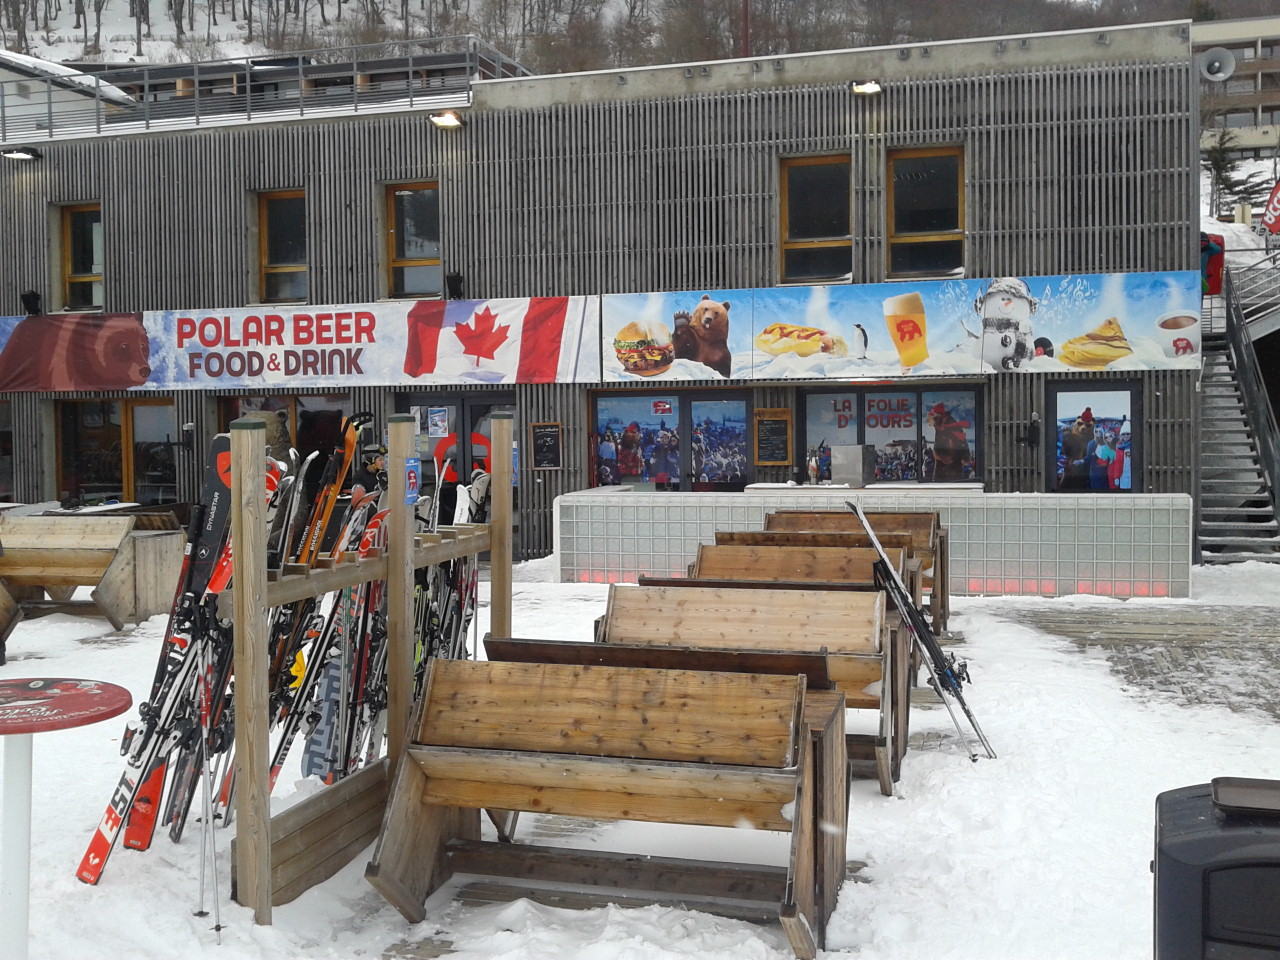
\includegraphics[scale=0.15]{PolarBeer.jpg}
\end{center}

\paragraph{} À la brasserie des pistes, il y avait le patron, la patronne au
bar, le cuistot, le pizzaiolo, et deux serveurs. Au contraire, au polar beer,
il n'y avait que deux serveuses. Cette différence s'explique par le
fonctionnement de chacun des établissements. En effet, étant servi à table à la
brasserie des pistes, il est nécessaire d'avoir plus de personnel qu'au polar
beer où les clients doivent aller chercher leurs consommations au comptoir. De
plus, dans chaque café la consommation est payée au moment de la prise en main
de celle-ci.

\paragraph{} Dans chacun des établissements il y avait une télévision. À la
brasserie des pistes, la télévision permet d'écouter RFM TV sauf au moment du
journal télévisé régional où l'on bascule sur France 3. Au contraire, au polar
beer, la télévision montrait des surfeurs et il y avait de la musique lounge en
fond sonore. On pouvait cependant remarquer que c'était surtout les adolescents
et jeunes adultes masculins qui regarder la télévision au polar beer quand
personnes ne regardait la télévision à la brasserie des pistes.

\paragraph{} La décoration de la brasserie des pistes était basique: des tables
carrées pour la partie restaurant et quelques tables rondes pour la partie bar,
des chaises en fer, quelques banquettes. Au contraire, au polar beer, la
décoration était moderne et humoristique: des tables hautes, longues ou rondes
avec des chaises hautes, les murs étaient principalement rouges avec des jeux
de mots par-ci, par là tels que ``beer crossing'' d'un côté du mur et ``bear
crossing'' de l'autre. De plus, le comptoir était séparé en deux parties
distinctes: le bar où des bouteilles étaient exposées juste derrière et une
partie snack servant uniquement les boissons chaudes, crêpes et gâteaux à cette
heure-ci.

\begin{center}
	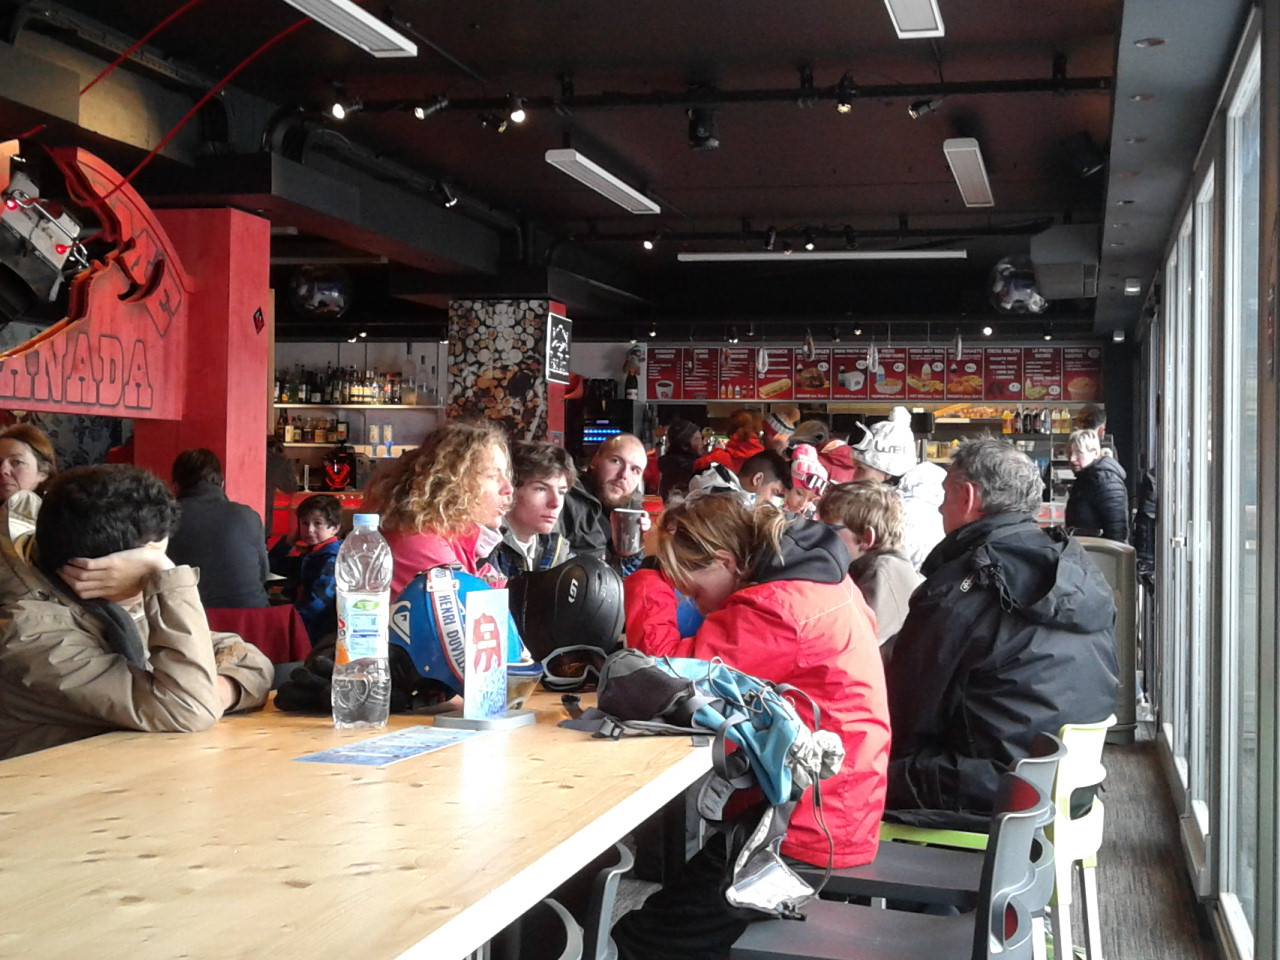
\includegraphics[scale=0.15]{PolarComptoir.jpg}
	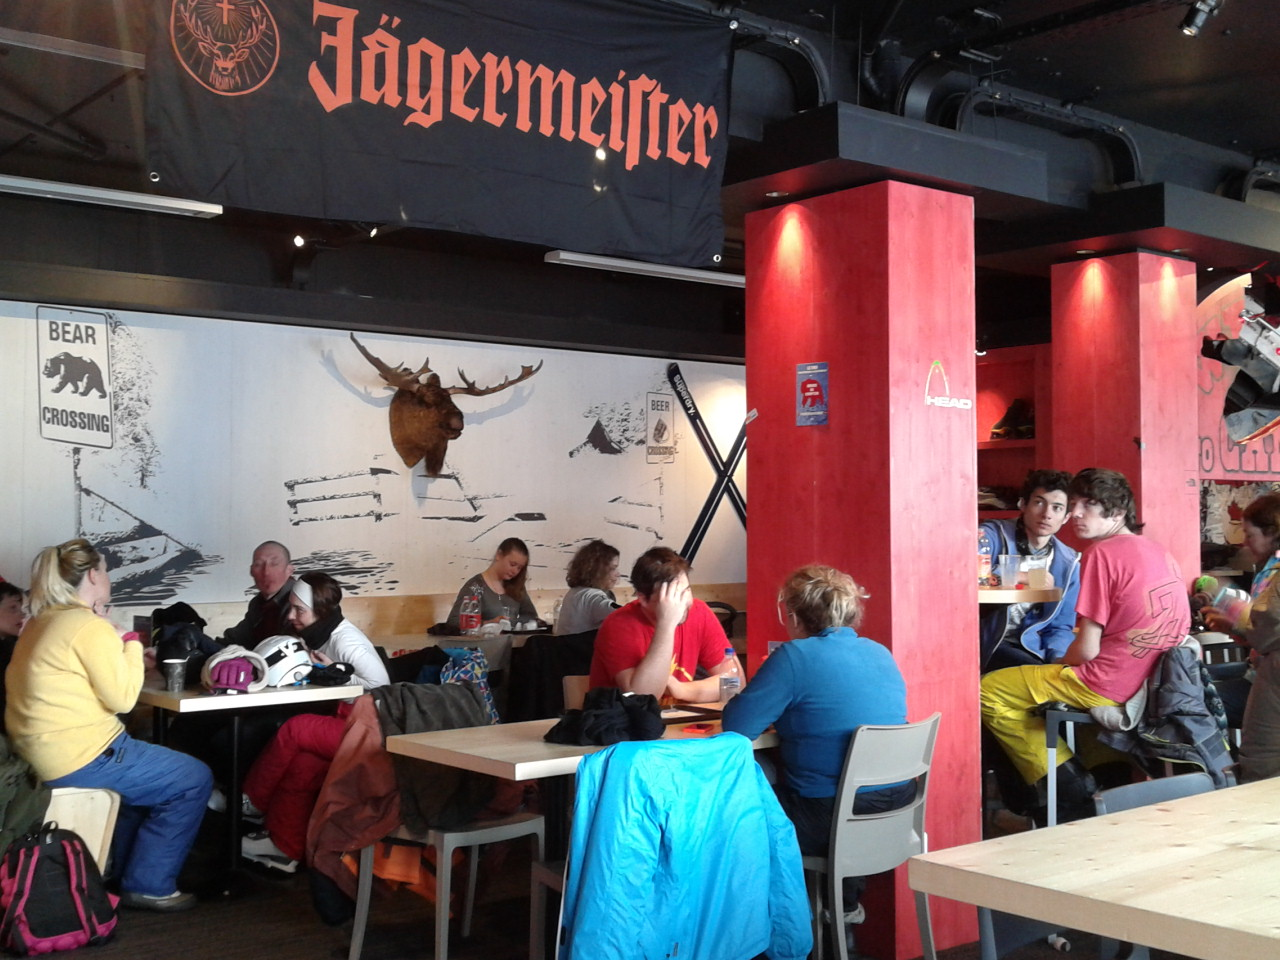
\includegraphics[scale=0.15]{PolarDeco.jpg}
\end{center}

\paragraph{} La population de chaque café était également différente.

\paragraph{} En effet, à la brasserie des pistes, il n'y avait personnes entre
18h45 et 19h00. Puis deux types de personnes sont arrivés peu à peu: il y avait
les familles avec enfants qui venaient diner et deux duos qui venaient boire un
coup. L'un des duos était des hommes d'environ trente ans qui ont pris chacun
deux vins chauds en jouant aux cartes. Le deuxième duo était un couple ayant
environ la soixantaine qui a également pris un vin chaud par personne. Ce choix
de boisson s'explique par la situation géographique du café: c'est une boisson
qu'on boit souvent au ski. Vers 19h30, la plupart des tables du restaurant
étaient prises par les familles avec enfants voulant diner. De plus, j'ai pu
remarquer que le comportement des serveurs variait avec les enfants: ils
prenaient un ton paternaliste et était aux petits soins. Enfin comme il
pleuvait et neigeait, la terrasse était vide.

\paragraph{} Au polar beer, la population était constituée de skieurs. Vers
16h, il s'agissait principalement de famille tandis que vers 16h45, la
population arrivante était principalement des groupes de jeunes adultes.
Certains restaient avec leur manteau et repartait après avoir bu leur
consommation et s'être un peu réchauffé. D'autres se déshabillaient un peu plus
et restaient plus longtemps. La principale consommation était des chocolats
chauds même si certains adolescents buvaient des sodas.  Certains sodas et la
bière étaient d'origine locale tel que l'``auvergnat cola''. Enfin, le soleil
étant au rendez-vous bien qu'un peu couvert, les fumeurs consommaient leurs
boissons et crêpes sur la terrasse tout en fumant.

\begin{center}
	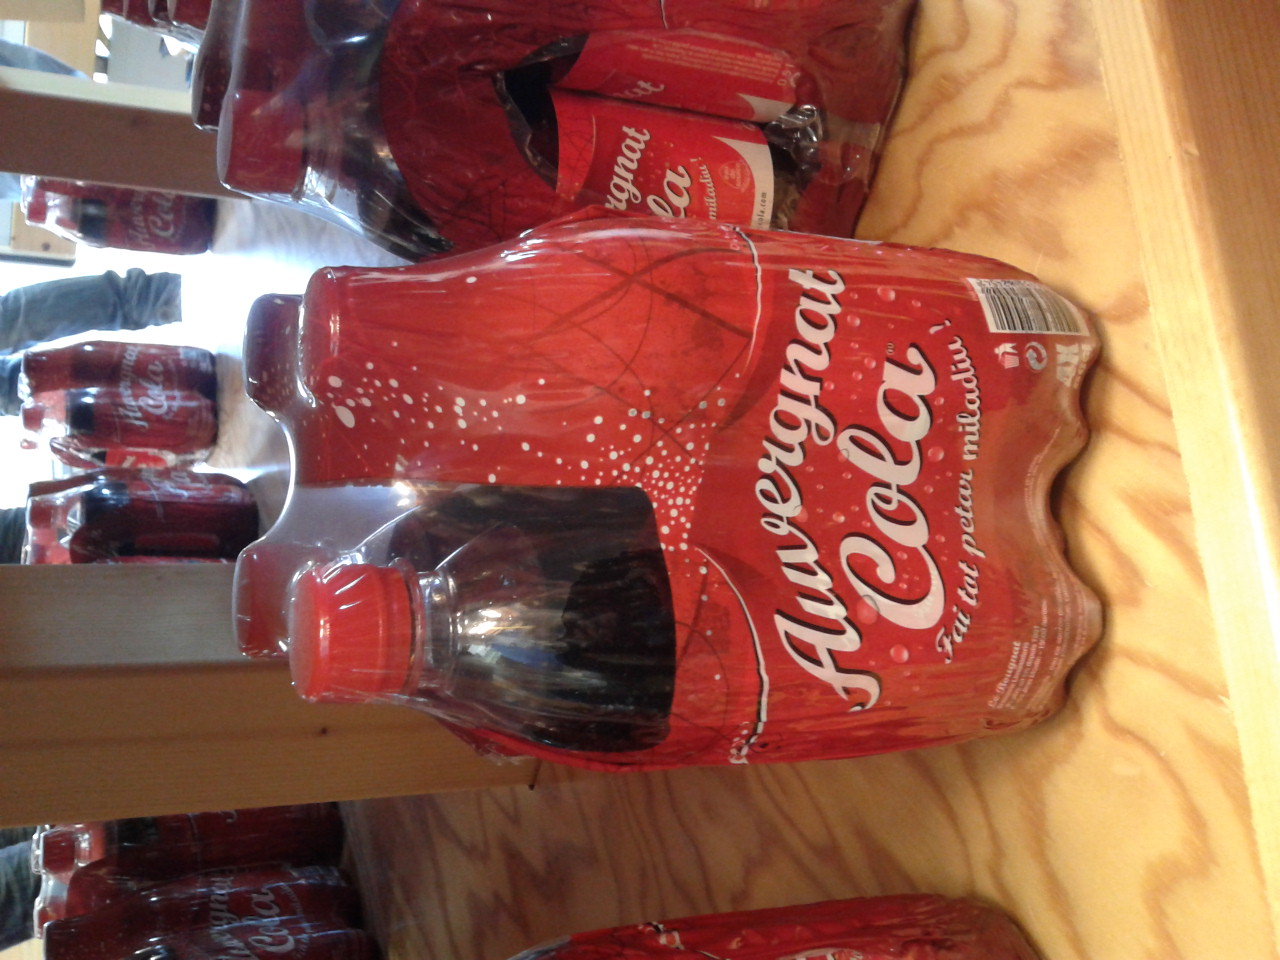
\includegraphics[scale=0.15,angle=270]{AuvergnatCola.jpg}
\end{center}

\paragraph{} De plus, si on compare la vie de ces deux cafés à celle d'un café
de campagne, on se rend compte que c'est encore différent.

\paragraph{} En effet, le vendredi, jour de marché, de 11h à 11h30 en août à
Arcis sur Aube, petite ville de 3000 habitants, le café et sa terrasse sont
bondés. Cette densité de population au sein de café est due au fait que les
habitués s'y retrouvent pour discuter des dernières nouvelles. Mon grand-père
étant un habitué, il s'arrête à chaque table pour dire bonjour aux gens qu'il
connait.  Puis il entre dans le café et dire bonjour au patron tout en
commandant un café. Ensuite, il va s'assoir avec une de ces connaissances, en
l'occurrence une grand-mère et ces trois petits enfants. La serveuse apporte le
café. Les petits enfants jouent au babyfoot pendant que les grands-parents
discutent des dernières nouvelles. Les personnes travaillant au café sont la
serveuse, le patron et son fils qui semble aider les jours d'affluence.

\begin{center}
	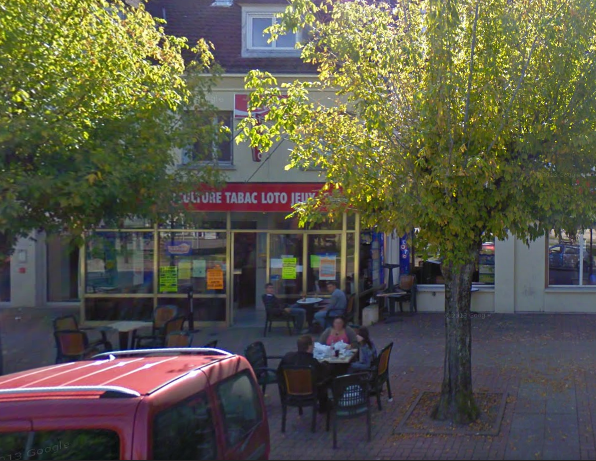
\includegraphics[scale=0.5]{BarArcis.png}
\end{center}

\section{2\ieme version}

\paragraph{}
\emph{Adams Café, Hammersmith, London}

\paragraph{} Le premier jour de printemps était arrivé, mais le froid était
toujours au rendez-vous. Près de la station Hammersmith, un quartier très
attractif du grand Londres, je me suis replié auprès du café Adams pour me
réchauffer.

\paragraph{} Très peu de temps après mon arrivée, une serveuse est venue vers
moi pour me proposer de boire un verre et de m'asseoir près de la grande baie
vitrée du café. Je lui répondis que je désire prendre un café avec un pancake
si cela était possible. Le café était très chic et décoré d'un bois rustique
qui me rappelait la bonne vieille époque.

\paragraph{} Je me suis donc assis à l'endroit qu'elle m'avait proposé, je
pouvais voir ces personnes qui couraient près du ``Tube Station'' de la station
d'Hammersmith, très utilisé de jour comme de nuit. Dans le café, beaucoup de
personne s'y trouvait, dont un couple de personne âgé qui m'a interpellé
accompagné de leur petit fils. Ils rigolaient et semblaient heureux d'être
ensemble.

\paragraph{} Au fond du café, un homme tout seul se trouvait là, je me
demandais ce qu'il faisait et pourquoi est-ce qu'il préférait être là, plutôt
que chez lui.  Réfléchissait-il à ce qu'il voulait faire dans la journée?

\paragraph{} Alors que j'observais les clients autour de moi, la serveuse
m'interrompit en me pausant mon café sur table en me souhaitant ``Have a good
lunch''.  Je la remerciais en la saluant pour lui dire qu'elle pouvait
disposer, car je n'avais besoin de rien d'autre que d'être seul.

\paragraph{} Pendant ce temps, un jeune couple entrèrent dans le café, avec des
sacs pleins les mains et des bagages sur le dos. À l'heure accent, j'en étais
sûr, c'était des Français. Je fus ravi qu'ils s'assoient à côté de moi, car je
me suis dit que je pouvais comprendre ce qu'ils disaient, sans même qu'ils ne
sachent que je comprenne ce qu'ils disaient.

\paragraph{} Ces dernières racontaient leur premier ressentis de leur voyage à
Londres et semblaient véritablement conquis par l'ambiance de ces lieux.

\paragraph{} Je déposais l'argent sur la table pour payer ce que j'avais
commandé, avec ce qu'on appelle un ``tips'', qui est un pourboire de 2 euros
que j'ai laissé pour cette charmante serveuse.

\paragraph{} Avant de partir, j'ai salué les 2 Français ``Have a nice day, dear
countryman'' et ils ont souris, ce qui m'a fait chaud au cœur, car moi aussi
j'étais heureux de me trouver à Londres.

\section{3\ieme version}

\paragraph{}
\emph{18 février, Le Pierrier, Châtel}

\begin{center}
	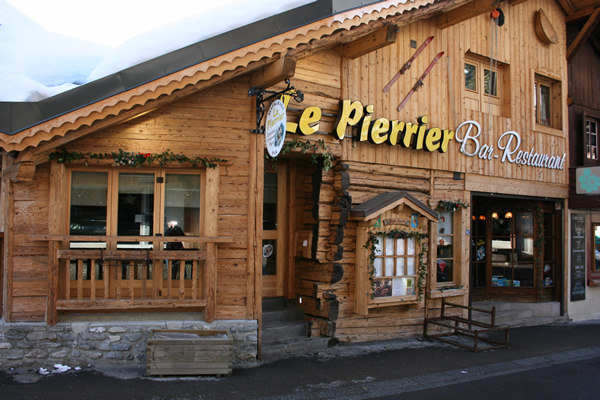
\includegraphics[scale=0.5]{pierrier.jpg}
\end{center}

\subsubsection{Introduction}

\paragraph{} J'ai fait mes observations dans le café de Châtel, pendant mes
vacances de ski.  Ainsi, il faut garder en mémoire que l'esprit des personnes
présentes dans le café est plus centré sur les vacances et donc l'ambiance est
très probablement plus joviale que la ``normale''.

\subsubsection{Différences ethniques}

\paragraph{} J'ai pu remarquer que les groupes entrant dans le café ne
possédaient pas beaucoup de différences ethniques. On peut donc supposer que
les groupes partant en vacances de ski (la plupart de manière familiale par
suppositions) le font la plupart du temps avec des personnes de la même ethnie.

\subsubsection{Consommations}

\paragraph{} Parmi les boissons consommées dans différents groupes, il existe
beaucoup de similitudes entre les consommations de chaque groupe. Par exemple,
un groupe entier consommera plus des bières en général alors qu'un autre groupe
consommera des boissons plus sucrées/chaudes comme des chocolats chaud ou des
cafés.

\subsubsection{Conversations}

\paragraph{} Pour des raisons de vie privées, je n'ai pas écouté avec précision
les conversations des personnes. Cependant avec des mots clefs, j'ai pu déduire
que les conversations tournaient en grande majorité autour du ski même
(performances, que faire ensuite). Sinon, les discussions tournaient souvent
autour des vacances.

\subsubsection{Positions}

\paragraph{} Des comportements récurrents que j'ai pu observer étaient que la
plupart du temps les hommes dans la tranche d'âge 20-40 se mettent souvent ou
presque toujours dans les coins ou dos à un mur, laissant aux enfants des
places avec chaises du côté où d'autres personnes, étrangères, passeraient.

\section{4\ieme version}

\paragraph{}
\emph{Jeudi 12 février, 8h25 – Café Cours des Roches, Noisiel}

\paragraph{} Je ne me sens pas à ma place, et en même temps je n'ai pas envie
de bouger. Un coup d'œil rapide à ma montre, huit heures vingt-cinq – trois
minutes, c'est bon, je peux attaquer mon chocolat chaud. Il n'y a rien de pire
que de se brûler la langue dans la précipitation. Mon croissant est déjà bien
entamé, mais de toute façon, je n'oserais pas le tremper dans ma tasse ; je
n'ai jamais su si c'était bien vu en public.

\paragraph{} Il y a dix minutes, je m'installais au café, commandais chocolat,
jus et viennoiserie, avec un léger trac. L'objectif: s'asseoir et observer.
Pas facile, quand on se sent soi-même en terre inconnue: je n'ai pas l'habitude
des cafés, et eux-mêmes n'ont sans doute pas coutume de voir un étudiant de 19
ans – moins en apparence – tout seul, balayer la salle un bloc-notes à la main.

\paragraph{} La salle est calme, peu remplie, les clients vont et viennent. La
plupart ne restent pas longtemps: nous sommes en face de la gare, et près de
toutes sortes de bureaux: trésor public, banque populaire\ldots On vient au
café des Roches pour y déjeuner sur le pouce, en attendant ou en sortant du
train.  Ou peut-être de ce cortège de bus dont les horaires ne se marient
jamais à ceux du RER. Je me félicite de ne pas être venu un jour de marché: la
place et les trottoirs y sont habituellement noirs de monde, alors je n'ose
imaginer l'atmosphère du bar.

\paragraph{} Je remarque tout de même des profils différents du cadre de
passage et du voyageur affamé. Au comptoir, quelques habitués venus partager
les dernières nouvelles avec le patron. J'y associe sans doute trop vite le
cliché habituel ; après tout, rien ne me dit qu'il s'agit du patron, d'ailleurs
je ne vois aucun torchon sur son avant-bras. Je ne saurais nommer le contenu de
leurs verres, mais il me semble plus éthylique que mon modeste jus d'orange.
Plus loin, à une table, un jeune couple sûrement trop tôt réveillé. Difficile
d'évaluer leur profession. Aspirés par leur conversation, ils délaissent leurs
boissons chaudes. Dans quel monde vivons-nous?

\paragraph{} Les quelques places en terrasse – un joli mot pour désigner le
trottoir – sont délaissées, sans surprise par ce froid.  J'aperçois un groupe
de trois lycéennes s'y asseoir, puis se raviser et entrer dans le bar. On leur
apporte vite des cafés. Rien d'étonnant, le lycée Gérard de Nerval est à deux
pas. Je me surprends à penser qu'elles sont un peu jeunes pour ce genre
d'établissement, avant d'estimer que je n'avais que deux ou trois ans de plus
qu'elles. On prend souvent un café parce que c'est une boisson de grand, et on
est trahi par la quantité de sucre, de lait et de mousse saupoudrée de cacao
qu'on y instille. Ça ne manque pas ici.

\paragraph{} J'en arrive à une conclusion: un café, c'est le lieu des grands
par excellence. Le lieu de ceux qui ont renoncé à un peu de sommeil
supplémentaire pour venir partager un verre, une tasse, un gobelet entre
collègues. La société plutôt que le rêve. Ce qui explique sans doute pourquoi
je ne m'y sentais pas à mon aise, et qu'un quart d'heure a suffi à me faire
penser que ces demoiselles devraient plutôt être en cours à huit heures et
demie. Une vraie réflexion de grand – c'est-à-dire de vieux.

\chapter{Communication Homme/Femme}

\paragraph{} Les hommes et les femmes ont une façon de communiquer très
différente. Cette communication varie également en fonction du sexe de leur
interlocuteur. En effet, les sujets de discussion et les façons de communiquer
verbalement et non verbalement ne sont pas les mêmes si les interlocuteurs sont
seulement masculins, féminins ou si les personnes qui discutent sont des deux
sexes. Nous avons donc observé et décrit des discussions au sein de ces
différents groupes.

\begin{center}
	
\includegraphics[scale=0.7]{h-f.png}
\end{center}

\section{1\iere version}

\subsection{Hommes}

\paragraph{} Les hommes sont hautement engagés dans la conversation, ils
parlent de leurs vies et de celle des autres dans les lieux qu'ils apprécient
et où ils y vont régulièrement. Leurs sujets de conversations sont généralement
les mêmes, on peut y retrouver leurs histoires personnelles avec leurs femmes,
ce qu'ils se passent à leurs lieux de travail ou leurs désirs. Dans leurs
conversations, beaucoup de sujet sensible qu'ils ne préfèrent pas que les
femmes entendent, parce qu'il s'agit de chose dont on ne doit pas en parler,
par pudeur vis-à-vis des femmes. C'est ce qu'on appelle ``parler de choses
tabou''.

\paragraph{} Concernant leurs façons d'interagir et de converser entre eux, on
peut remarquer qu'ils sont très réactif face à toutes leurs remarques et
n'hésitent pas à s'imposer face aux autres. Leurs mécontentements face à une
remarque pour montrer leurs mécontentements peut prendre des proportions
disproportionné. Il n'y a aucune diplomatie dans leurs conversations.

\paragraph{} On peut comprendre qu'ils sont dans une logique de supériorité et
qu'ils cherchent toujours à être au-dessus des autres. En effet, les hommes
sont sensibles dans les interactions à créer une dynamique de pouvoir et ils
parleront de façon à permettre une différenciation entre les dominants et les
dominés.

\paragraph{} Ces discussions ont eu lieu au Mac Donald's avec un groupe d'amis,
un vendredi soir après le boulot pour certains et les cours pour d'autres. Ces
petits moments de retrouvaille sont hebdomadaire et font partie de notre
routine.

\paragraph{} Par rapport aux conclusions de Deborah Tannen, je trouve que les
hommes cachent soigneusement leurs doutes. En effet, ils considèrent que c'est
se mettre dans une position de faiblesse et seront toujours attentif à ne pas
se mettre en situation d'infériorité.

\subsection{Femmes}

\paragraph{} Les femmes sont hautement respectueuses du locuteur. Les femmes
conversent de leurs mœurs et des conduites individuelles.  Ces sujets sont
très intéressants pour ces personnes, car elles sont très curieuse de découvrir
la vie de leurs amies. Les histoires d'amours, les livres qu'elles ont lus
récemment, les films et séries qu'elles ont adorés, beaucoup de sujet de
conversation sont à noter de leurs côtés.

\paragraph{} Bien que les conversations sont denses et sans arrêt, ce qui me
surprend c'est que personne ne se coupe la parole et toutes les personnes
respectent l'opinion du locuteur. Dans les rituels de conversation des femmes,
les femmes utilisent beaucoup plus fréquemment les formules de politesse et
d'excuse que les hommes comme ``Je suis désolée''. Parmi ce rituel, il y a
aussi l'échange de compliment que les femmes se font de façon réciproque.

\paragraph{} C'est une façon de continuer le dialogue pour ne pas laisser ce
qu'on appelle ``un blanc'', en minimisant ses propres qualités sur un mode qui
implique que l'autre en reconnaîtra le caractère et aura la possibilité de lui
adresser un compliment en retour.

\paragraph{} Ces discussions ont lieu au Starbuck avec le groupe d'amie
qu'elles gardent depuis les années du lycée.  Comme pour les hommes, c'est en
soirée le vendredi soir, la veille du week-end. Ce sont aussi des retrouvailles
hebdomadaire.

\paragraph{} Par rapport aux conclusions de Deborah Tannen, les femmes feront
attention à l'autre concernant la domination. En effet, les femmes apprennent à
minimiser les signes qui indiquent la supériorité de l'une sur les autres.
Elles prônent l'égalité entre elles.

\subsection{Mixtes}

\paragraph{} Bien que nous ayons remarqué que les hommes et les femmes avaient
différente culture de communication, jusqu'au point de qualifié ces
conversations de ``multiculturelle'', on remarque qu'on peut parler de la même
chose que dans les groupes composé uniquement d'homme ou femme, mais il y a des
répercussions sur les jugements de compétence, de confiance en soi qui sont
portés sur les personnes. En effet, ce que nous apprenons par la culture des
autres nous apprend à juger et à évaluer les autres par rapport aux autres.
Notamment par la directivité du message, les temps de pause et le choix des
mots.

\paragraph{} Les conséquences sont que les femmes vont dire ``nous'' et les
hommes employer le pronom ``je''. La principale problématique à ce jour dans
le monde du travail, c'est la prédominance de certains face à d'autres. C'est
la raison même de la venue du sexiste, car chaque personne a été catégorisé et
de nombreux mouvement tente de mettre fin à cette complication dans la sphère
du travail.

\paragraph{} Les femmes et les hommes sont bien égaux, ce n'est que leurs
cultures et façon de faire qui sont différente.

\section{2\ieme version}

\paragraph{} Dans chaque cas, je suis restée à distance en position
d'observatrice.

\subsection{Hommes}

\paragraph{} Les deux groupes masculins ont été observés dans le RER, le
premier, samedi à 17h45, et le deuxième, dimanche à 21h.

\subsubsection{groupe A}

\paragraph{} Il s'agissait d'un groupe de trois personnes où principalement
deux des trois participait à la discussion. Lorsqu'ils parlaient des drones,
ils se sont penchés sur un téléphone portable pour illustrer leur discussion.
Puis ils ont parlé d'un sport tout en faisant des imitations pour illustrer
leurs propos. L'un d'entre eux a souri alors qu'il parlait d'un partiel qu'il a
tout juste réussi ce qui l'a embêté. Ensuite ils ont discuté des difficultés
qu'ils rencontreront l'année prochaine dans leurs études. Lors de cette
discussion, l'un d'eux à donner une tape sur l'épaule de l'autre pour lui
montrer son soutien. Durant toute leur discussion, ils se sont rarement regardé
les uns les autres.

\subsubsection{groupe B}

\paragraph{} J'ai pu observer dans le RER deux hommes qui se sont croisés par
hasard. Ces deux hommes se connaissaient de longues date mais ne s'étaient pas
vu depuis un moment. Ils se sont serrés la main et ont échangé les dernières
nouvelles. Durant cette discussion, ils ne se sont que très peu regardé comme
le groupe précédent.

\subsection{Femmes}

\paragraph{} Pour les groupes féminins, l'observation a eu lieu dans un bar
entre 21h et 22h.

\subsubsection{groupe A}

\paragraph{} Il s'agit de deux filles. L'une se plaint d'un homme tandis que
l'autre l'écoute et lui donnes des conseils de temps à autre. La fille qui est
écoute est adossée à son dossier tandis que l'autre est penché sur la table. De
plus, la fille qui se plaint joue avec des objets tels que son bracelet ou un
élastique. La plainte de la fille est ponctuée de gestes amples et de beaucoup
d'intonations.

\subsubsection{groupe B}

\paragraph{} Dans ce cas, il s'agit de trois filles se trouvant un peu trop
loin pour que je puisse comprendre toute la conversation. L'une d'entre elles
était en train de parler d'un problème qu'elle rencontrait pour se loger
pendant que les deux autres écoutaient. La fille qui parlait faisaient de grands
gestes et parlait fort avec beaucoup d'intonation. Elle était penchée sur la
table tandis que les deux autres étaient adossées à leur dossier.

\subsection{Mixtes}

\paragraph{} Pour les groupes mixtes, l'observation a eu lieu dans un Fast Food
entre 19h30 et 20h30. Je n'ai donc pu observer que des binômes. Dans chacun des
cas, je n'ai pas pu entendre de quoi ils parlaient à cause de la distance.
Cependant, j'ai pu imaginer le type de conversation grâce au langage corporel.

\subsubsection{couple A}

\paragraph{} Le couple est assis face à face, surement pour faciliter la
communication. L'homme, bien qu'ayant fini de manger, est penché vers la fille
au-dessus de la table. Ses mains sont coincées sous ses jambes ce qui est un
signe de stress. La fille, quant à elle, est en retrait appuyées sur le dossier
de sa chaise. Elle est restée souriante tout au long du repas. L'homme ne peut
s'empêcher de la regarder tout le temps même lorsqu'il a débarrassé les
plateaux. On peut donc en déduire que ces personnes sont très proches. En
effet, l'homme voudrait plus que de l'amitié tandis que la fille ne le
considère que comme un très bon ami.

\subsubsection{couple B}

\paragraph{} Le couple ne se situe pas face à face, ils se sont positionnés en
diagonale. Ils ne se regardent jamais. La fille utilise ses écouteurs pendant
que l'homme regarde son portable. Seul l'homme mange, la fille n'a pas de
plateau. Lorsque l'homme part, la fille le regarde dans le dos en levant les
yeux au ciel ce qui confirme qu'ils se connaissaient. On peut donc en déduire
qu'ils sont en froids et on peut même supposer qu'ils viennent de rompre. Puis
un deuxième homme rejoint la fille. À ce moment son attitude change du tout au
tout: elle sourit, elle joue avec ses cheveux, elle le regarde sans arrêt. On
peut donc en déduire qu'elle est en de bien meilleurs termes avec cet homme et
on peut même supposer qu'elle souhaite le séduire.

\subsection{Conclusion}

\paragraph{} Suite à ces observations, j'ai pu me rendre compte que les femmes
ont une interaction physique entre elles bien plus fréquente qu'entre les
hommes: elles se regardent tout au long de la conservation contrairement aux
hommes, les hommes se soutiennent tout en restant à distance comme le montre la
tape sur l'épaule qui est un geste très bref et assez éloigné du reste du
corps. Les hommes parlent souvent de technologies ou de sport tandis que les
femmes se plaignent généralement des problèmes qu'elles rencontrent dans leur
vie. De plus, les hommes ont tendance à illustrer leurs propos alors que les
femmes occupent leurs mains pendant leurs conversations. Enfin, dans les
groupes mixtes, l'attitude des gens varie du tout au tout entre les moments où
ils veulent séduire leur partenaire et les moments où ceux-ci ne les
intéressent pas du point de vue séduction.

\paragraph{} Comme l'affirme D. Tannen, les femmes s'écoutent parler sans
s'interrompre et écoutent les conseils donnés sans problème. De même, les
hommes tentent de rester en position de force avec des gestes ``viril'' comme
la tape sur l'épaule.

\section{3\ieme version}

\paragraph{} La psychologie variant indubitablement de manière prononcée de
personne en personne, il me semble judicieux de préciser auparavant que mes
observations sont sujettes au biais d'échantillonnage, ne constituent pas un
échantillon suffisant de la population et ne sont donc pas des observations
représentative de la majorité.

\subsection{Hommes}

\paragraph{} Le cas no 1 est le cas général des discussions à la cantine. Étant
assis, l'analyse du langage corporel est assez difficile. Cependant j'ai
remarqué une certaine tendance chez les “hommes” de la table à faire plus de
blague “moqueuses”, dépréciant de manière humoristique les caractéristiques
d'une personne (homme ou femme). Si la blague est réussite, une partie des
hommes considèrent momentanément et toujours de manière humoristique la
personne comme ayant un statut supérieur à ce qu'il était auparavant ou
supérieur aux autres personnes, notamment la personne ciblée par la
plaisanterie. Bien que ce soit humoristique, il semblerait que ce comportement
soit plus profond qu'il n'y paraît.

\subsection{Femmes}

\paragraph{} Le cas no 2 est lors des sorties “Bières du Club” organisées par
le Club *Nix.  J'ai remarqué lors de ces sorties que les femmes avaient plus
tendance à exprimer ce dont elles ressentent et ce qu'elle pense alors que les
hommes avaient tendance à parler de faits et d'actions.

\subsection{Mixtes}

\paragraph{} Le cas no 3 est lors des discussions en amphithéâtre. Les
discussions lors de ces moments sont plus orientés “cours” car les élèves sont
à ces moments là focalisé sur leurs études. J'ai remarqué qu'en général
(contrairement à mon opinion initiale) les hommes sont plus enclins à demander
de l'aide à d'autres personnes dans l'amphithéâtre alors que les femmes préfère
se “débrouiller” de par elles-mêmes et travailler à la maison/appartement.

\chapter{Entretiens}

\paragraph{} Le choc des cultures est courant pour toute personne restant un
certain temps dans un pays étranger. En effet, une personne arrivant dans un
pays étranger possède des a priori sur ce pays qui seront remis en cause par
leur expérience dans ce pays. Voici des témoignages de personnes étrangère
ayant vécu en France pendant un long moment.

\begin{center}
	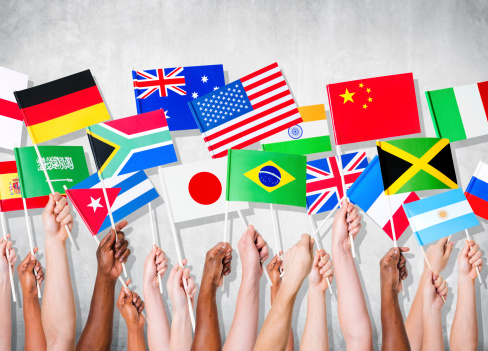
\includegraphics[scale=0.5]{entretien.jpg}
\end{center}

\section{1\iere version}

\paragraph{} Dans le cadre de l'exploration ``entretien avec un étranger'',
nous avons discuté avec deux personnes différentes à savoir Carmen Matellan,
professeur d'espagnol, et Catherine, stagiaire de l'épi 2.

\paragraph{} Madame Matellan est arrivée en France il y a 25 ans pour se marier
et fuir la dictature. Sa vision de la France a été modifiée après son arrivée.
En effet, elle voyait la France comme le pays de la liberté, l'égalité et la
fraternité. Cependant, elle s'est rendu compte que ce n'était pas un pays si
fraternel et égalitaire que prévu: les études poursuivies sont décidées suite à
un concours, toutes les études ne sont pas accessibles à tous à cause de leur
coût, la vie est bien plus hiérarchisée qu'en Espagne du temps de la dictature.

\paragraph{} Les différences flagrantes entre l'Espagne et la France sont dans
les horaires, la nourriture et le pessimisme français opposé à l'optimisme
espagnol. Cette différence entraine des difficultés. En effet, elle est souvent
prise pour une simplette à cause de son sourire constamment présent. De plus,
elle trouve que les Français sont un peu hypocrite dans leur politesse et dans
leur manque de solidarité: ils se permettent tout et n'importe quoi à partir du
moment où ils s'excusent notamment dans le métro.

\paragraph{} Elle est émerveillée tous les jours par la beauté de Paris et la
culture française telle que l'histoire, la littérature ou la beauté de la
langue elle-même. C'est pourquoi elle est choquée par le faible niveau de
français des jeunes. En effet, beaucoup de jeunes font de nombreuses fautes de
français et détruise ainsi la langue.

\paragraph{} Catherine est une étudiante arrivée en août dernier pour faire un
stage d'un an. Elle s'occupe de créer les listes de présence des groupes de
langue. Elle vient de la banlieue Londonienne. Elle a décidé de venir en
France pour améliorer son français. En effet, elle étudie la philosophie et le
français à l'université de Liverpool.

\paragraph{} Avant de partir, elle pensait que Paris était plus propre et plus
grand. Elle pensait aussi se faire plus d'amis français avec qui discuter.
Elle trouve que les gens sont mieux habillés en France et que la vie est plus
chère. Enfin,  elle a été surprise plusieurs fois par le fait que des hommes
l'ont suivi dans la rue ce qui lui a fait un peu peur.


\section{2\ieme version}

\paragraph{} Takamichi Ishii est un étudiant japonais de 22 ans arrivé en
France en février. Il a étudié deux mois à l'ESIEE avec des compatriotes et a
accepté de répondre à nos questions. À sa demande, nous l'appelions Taka - il
nous a confié être appelé différemment par chacun de ses camarades. Si le
niveau de familiarité en France se distingue par l'usage du prénom et du
tutoiement, on trouve en japonais de nombreuses façons d'appeler quelqu'un, en
utilisant des suffixes comme -kun ou -san ; le prénom seul n'est utilisé que
par les proches.

\paragraph{} Taka est parti de Kanagawa (près de Tokyo) pour un voyage d'études
et a choisi la France pour sa renommée touristique. Il nous a confié apprécier
notre pays et vouloir y rester plus longtemps. Nous l'avons interrogé sur la
prétendue impolitesse des Français, dont on parle beaucoup dans les médias,
mais Taka nous trouvait au contraire plutôt agréable. Second cliché évincé:
selon lui, les Français parleraient selon lui un bon anglais, bien meilleur en
tout cas  que celui des Japonais ; ce qui était un avantage puisque la langue
française lui paraissait très complexe. Nous serions surtout moins timides
qu'eux, ce qu'il considérait comme une qualité (nous en étions moins sûrs).

\paragraph{} Un point négatif tout de même: la région parisienne lui a paru
sale, du RER aux bords de routes en passant par les sanitaires. Il faut dire
que, selon Taka, les Japonais sont plus surveillés. Lorsque nous lui avons
demandé de se rappeler un évènement qui l'avait choqué, il a tout de suite
évoqué les fraudeurs du RER. Il est impossible au Japon de sauter par-dessus
les portiques, puisque les gardiens n'hésitent pas à intervenir ; il était
déconcerté de voir les employés de la RATP rester passifs, désabusés.

\paragraph{} Nous en sommes venus à parler du choc des cultures: Taka estime
que tout est différent entre les quotidiens européen et japonais. On vient de
l'évoquer: si nous nous plaignons de l'augmentation de la surveillance, elle
reste bien moins importante qu'au Japon. Une conséquence, sans doute: les
pickpockets sont beaucoup plus répandus chez nous, ce qui l'a surpris: l'un de
ses amis s'était déjà fait voler son téléphone. Les trains sont bien plus
souvent en retard. Taka nous a également parlé de différences plus triviales,
mais qui lui avaient sauté aux yeux: la rareté des distributeurs automatiques,
qui au Japon sont parlants, vendent de tout et surgissent tous les deux mètres
; les Français peuvent garer leur voiture sur le côté de la rue et pas
uniquement dans des parkings ; les rues portent des noms de célébrités, et pas
seulement des numéros.

\paragraph{} En somme, ce qui frappe le plus les Japonais en France, ce sont
les détails ; ceux qui font que malgré une grande occidentalisation de la
culture japonaise, le quotidien reste toutefois très différent.


\chapter{Dislocations}

\paragraph{} Il n'est pas toujours nécessaire de changer de pays pour sortir de
notre zone de confort et d'habitudes. En effet, voici nos témoignages sur ces
moments où nous sommes sorti de notre zone de confort. Nous y avons décrit nos
pensées et nos sentiments tout au long de cette expérience.

\section{1\iere version: Les femmes et les soldes}

\begin{center}
	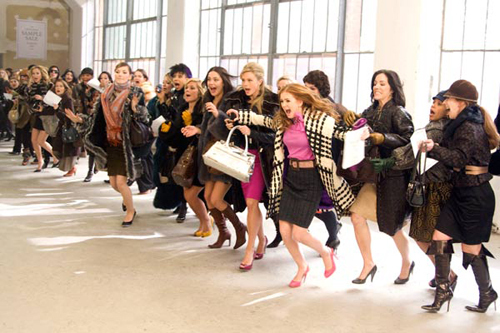
\includegraphics[scale=0.7]{solde.jpg}
\end{center}

\paragraph{} J'ai décidé, pour ma situation de dislocation, de raconter mon
expérience, entourée d'un groupe féminin en furie. Je me suis donc dirigé dans
un magasin de femme lors des soldes d'été. J'étais partie au magasin Zara for
Woman le 25 juin et je me suis rendu compte que les vêtements pouvaient rendre
folles les femmes. Je les contemplais, se déchirer les habits pour la dernière
taille et courir partout pour trouver la robe parfaite.

\paragraph{} Le temps passa et de plus en plus de femme venait dans la boutique
pour y faire leur shopping et trouver de bonne affaire. Toutes les femmes
vinrent dans cette boutique qui attirait aussi bien les jeunes femmes que les
adultes accompagnés de leurs enfants. Aucun homme n'était là, car ils étaient
dans le magasin d'en face, à Zara for Men.

\paragraph{} Cet environnement de femme fut nouveau pour moi, car nous
entendions que des voix aigües accompagné des bruits des caisses et des
vendeurs. En faisant le tour du magasin et regardant les articles, j'ai
commencé à écouter des bouts de conversation des passantes.  Nombreuses sont
celles qui ont dit faire des affaires de folie et sont pressé d'aller dans
d'autres magasins. Un autre groupe parlait de où est-ce qu'elles pourraient
aller discuter autour d'un café ou d'un Starbuck.

\paragraph{} Je n'étais pas du tout dans mon environnement et le temps semblait
passer pourtant très vite, c'était une expérience à refaire, car très marrante!

\section[2\ieme version: l'avion]{2\ieme version: la première fois que j'ai pris l'avion toute seule}

\begin{center}
	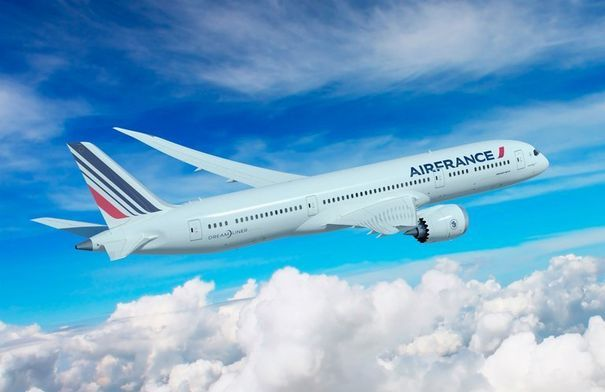
\includegraphics[scale=0.6]{avion.jpg}
\end{center}

\paragraph{} La première fois que j'ai pris l'avion toute seule fut pendant ces
vacances. J'avais déjà pris l'avion mais toujours avec quelqu'un en me laissant
guidée. J'étais donc légèrement anxieuse à ce sujet. C'était d'autant plus vrai
que je savais que la première fois que mon frère avait pris l'avion tout seul,
il s'était trompé à un moment et était passé à travers les contrôles de
sécurité. J'avais donc un peu peur de faire la même erreur que lui. J'ai donc
fait tout le trajet jusqu'à l'aéroport en regardant l'heure toutes les deux
minutes de peur d'être en retard: on ne sait jamais ce qui peut arriver avec
les transports en commun.

\paragraph{} Je suis donc arrivée à l'aéroport sans problème. J'ai repérer où
je devais aller ensuite pour embarquer puis je suis allée m'acheter à manger vu
qu'il était au environ de midi et que j'avais encore au moins une heure de
marge avant l'embarquement. Je me suis occupé en jouant sur une application
pendant que je mangeais: je me sentais seule et toujours aussi anxieuse en
pensant aux contrôles de sécurité à passer.

\paragraph{} Je me suis approché des contrôles de sécurité sans trop savoir si
je devais les passer maintenant ou attendre un peu: j'avais pas mal de temps
devant moi avant l'heure de l'embarquement. Je me suis donc décidée à demander
conseil à une employée de l'aéroport. J'ai eu quelques difficultés à l'aborder
: je n'étais pas la seule à tenter de la solliciter. Lorsqu'elle m'a enfin
accordé son attention c'était pour me dire ``vous pouvez passer quand vous
voulez''. N'ayant rien d'autre à faire je me suis exécutée et j'ai passé les
contrôles de sécurité sans aucun problème.

\paragraph{} J'ai ensuite essayé de repérer la porte d'embarquement de mon vol.
Une fois celle-ci repérer, je me suis assise proche de celle-ci en attendant
l'heure de mon embarquement: j'ai encore une fois regardé l'heure toutes les
deux minutes tout en vérifiant les panneaux affichant les portes d'embarquement
pour chaque vol. Tout à coup je me suis rendu compte que la porte avait changé.
Je suis donc restée deux minutes à réfléchir si je devais bouger ou pas en me
demandant si ça n'allait pas encore changer. J'ai fini par m'approcher de la
nouvelle porte indiquée. Je suis restée debout en attendant l'heure de
l'embarquement: il n'y avait plus énormément de temps à attendre et je n'étais
pas sure du fait qu'il n'y aurait pas un autre changement de porte à la
dernière minute.

\paragraph{} Une fois l'embarquement commencé, toute anxiété s'est envolée: je
retournais dans un environnement déjà connu.

\section{3\ieme version: Parler en public}

\paragraph{} Étant une personne peu à l'aise en public et assez timide quand il
s'agit de partager des opinions, quand l'on m'évoque rien que la combinaison
des deux il m'arrive d'être mal à l'aise rien que d'y penser. Quand bien même,
j'ai décidé de l'essayer et de surmonter mes peurs.

\paragraph{} À l'occasion d'une mauvaise expérience, j'ai décidé de réunir des
personnes, de partager mes opinions et d'organiser une discussion. Étant devenu
l'organisateur, je n'avais pas d'autre choix que de devenir le centre
d'attention de ce comité. Il s'agissait d'un situation très désagréable pour
moi au début. Cependant, au fur et à mesure que les personnes discutaient, je
me sentais de plus en plus à l'aise dans cette situation car ces personnes,
voyant que j'étais stressé, arrivaient à me faire comprendre qu'il n'y avait
aucune raison de l'être et qu'ils n'avaient pas de problème avec ma personne.

\paragraph{} Finalement, je garde un bon souvenir de cette expérience et pense
que cela va m'aider à me sentir plus à l'aise dans le futur, ce qui sera un
grand avantage par rapport à mon précédent moi.

\section[4\ieme version: le mariage]{4\ieme version: un mariage entouré d'inconnus}

\paragraph{} Étant le dernier de ma famille, je ne suis pas proche de mes
cousins dont certains se rapprochent dangereusement de la trentaine. Nous
passons peu de temps ensemble, donc je ne sais pas vraiment comment ils me
voient, ou ce qu'ils pensent de moi. J'ai été invité au mariage du plus ancien
d'entre eux, ce qui m'a poussé à m'impliquer davantage dans la famille étendue,
au moins pour une soirée. Heureusement, il y a quelque chose de mystérieux dans
ce genre de fête, qui permet à tout le monde de discuter sans connaître
vraiment son interlocuteur. Serait-ce le champagne? Alors que je pensais que
ma timidité me garderait en sécurité avec mes frères et sœurs, je me suis
surpris à discuter avec plus de monde, et sans hésitation.

\paragraph{} L'expérience se déroulait donc plutôt bien, de la messe à
l'apéritif, jusqu'à ce que mon cousin m'interpelle. Il m'apprit que, pour le
dîner, j'avais été placé à une table où je ne connaissais personne ; au
contraire de mes frères et sœurs, ce que j'appris plus tard. Mais, me
rassura-t-il, ``ce ne sont que des gens comme toi''! Charmant. Qu'est-ce que
cela pouvait vouloir dire? De sa part, j'imaginais qu'il s'agissait d'amateurs
d'informatique, mais cela pouvait-il remplir toute une table? Je pense avoir
compris la manœuvre: on avait dû dire dans la famille que je n'étais pas du
genre à profiter du mariage pour discuter avec les invités que je ne
connaissais pas, et le marié a cru de son devoir de m'y pousser. Pensant fort à
mon devoir de MSH, j'acquiesçai et me rendit, peu rassuré, au dîner, pour y
découvrir finalement que “des gens comme moi” signifiait “des lycéens”. Tous de
la famille de la mariée, ils se connaissaient et, fatalement, se comprenaient
assez pour que je sois perdu dans les conversations. Je me sentis glisser peu à
peu de cette fameuse zone de confort, le summum étant le moment où chacun
entonna à tue-tête un hymne bourguignon, celui-là même qui coûta à Messieurs
Montebourg et Hamon chantaient en septembre dernier.  Les plats débarrassés, la
tablée se dispersa assez vite et je rejoignis ma famille. J'avais ainsi vécu
une expérience à double tranchant: redoutant la foule, je m'y étais finalement
immergé de plein gré et sans trop de mal durant l'apéritif tandis que la
seconde immersion, contrainte, fut beaucoup moins positive. Peut-être était-ce
dû à la contrainte, ou alors simplement au fait que je rejoignais à table un
groupe déjà formé.


\chapter{Enfants}

\paragraph{}
Les enfants ont un fonctionnement qui leur est propre. De ce fait, un groupe constituer d'enfants forme une micro-société différente de celle des adultes. Celle-ci est dirigé par les enfants les plus agés au caractère le plus fort comme nous avons pu l'observer dans les parcs.

\begin{center}
	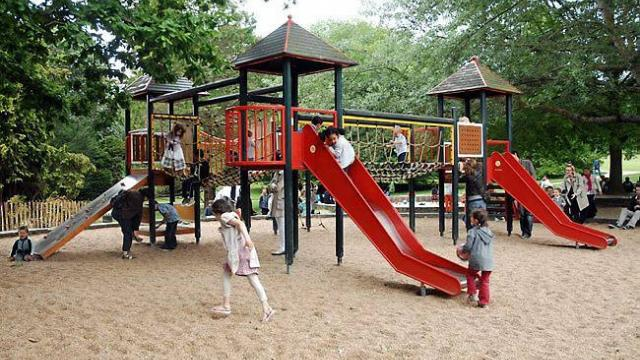
\includegraphics[scale=0.7]{enfants.jpg}
\end{center}

\section{1\iere version}

\paragraph{} Il faisait beau ce jour-là, nous étions le samedi 25 avril 2015 à
Bussy-Saint-Georges. Cette magnifique ville a le mérite d'être verte et de
disposer de nombreux lacs, parc et verdure.

\paragraph{} Après un bon footing matinal et un déjeuner au premier restaurant
copieux du coin, j'ai décidé d'aller me promener. Les oiseaux chantaient et le
vent faisait des caresses sur la peau, c'était donc le temps parfait pour les
enfants de jouer dehors et aux parents de se ressourcer après une semaine de
travail.

\paragraph{} Le parc à côté du lac appelé ``île mystérieuse'' était donc
l'endroit parfait pour réaliser l'expérience sociale d'observer des enfants
dans un parc.

\paragraph{} Je marchais, très lentement, car je regardais le ciel et ses
avions en train de voler, venant de pays si lointain, comme la Chine ou
l'Amérique. Une fois arrivé près du lac, j'ai fait le tour avant de trouver un
banc où personne n'était assis dessus.

\paragraph{} Une fois assis, je me suis mis à contempler le paysage, regarder
les signes de l'autre côté, puis j'ai commencé à me focaliser mon regard sur le
parc. J'y voyais des enfants courir dans tous les sens, un groupe de garçon
était en train de jouer au ballon tant dis qu'un groupe de fille jouait à la
marelle. Les enfants étaient très nombreux aujourd'hui et nous pouvions y
distinguer quelques un beaucoup plus sage que d'autres.

\paragraph{} En effet, j'observais un groupe de jumeau collé à leur mère et un
autre qui courait partout, sa mère ne pouvait même pas le rattraper. C'est
alors qu'un enfant turbulent a commencé à tomber par terre et s'est mis à
pleuré si fort que tout le monde le regardait. Très vite, un autre enfant est
venu le voir pour l'aider et essayer de guérir son bobo.

\paragraph{} Près d'ici, je décidai d'avancer vers un parc à côté où se
trouvait des jeux extérieur, notamment ce château en plastique où les enfants
s'amusent à escalader pour faire le toboggan. Je les regardai, tous heureux
d'être là, de remonter et redescendre sans cesse. Une joie les prenait
lorsqu'ils glissaient jusqu'en bas. De nombreuses mères se trouvaient là et je
décidai de discuter avec elles.

\paragraph{} J'ai fait connaissance de Nathalie dont son enfant jouait à
attraper les petits insectes près du château. Je remarquai que tous les enfants
étaient différents et d'autres plus joyeux que d'autres. En effet, son deuxième
enfant, Sophie, se trouvait près d'elle et ne voulait pas jouer avec les
autres.

\paragraph{} Cette expérience a été très enrichissante et une véritable ouverte
vers d'autres personnes car j'ai pu faire la connaissance d'une
Buxangeorgienne.

\section{2\ieme version}

\paragraph{} J'ai fait ces observations un dimanche après-midi du mois de mai.
Ce jour-là, il faisait très beau. La population du parc était donc assez
nombreuse.

\paragraph{} Dans une partie du parc, il y avait un terrain de foot comme on
voit souvent dans les banlieues: des cages pour les buttes surmontées de panier
de basket si des gens souhaitent jouer au basket. Le terrain était surtout
occupé par des adolescents de sexe masculins. Certains jouaient tandis que
d'autres observaient la partie accoudée ou assis sur les barrières délimitant
le terrain. J'ai pu remarquer que ces garçons avaient l'air d'être plutôt
sportif.

\paragraph{} De l'autre côté du parc, il y avait des transats sur lesquels des
adolescentes discutaient en bronzant. Sur les transats, j'ai également pu
observer des adultes en train de lire des livres tout en jetant un coup d'œil
aux enfants jouant sur les jeux.

\paragraph{} Les plus jeunes enfants, d'environ 3 ou 4 ans, jouaient sur un
toboggan sous la surveillance rapprochées de leurs parents. En effet, ce
toboggan possédant des parties à escalader, les enfants risquaient de tomber et
de se blesser. De plus, certains de ces enfants avait un équilibre pas très
bien développé et avaient parfois besoin d'aide pour passer certains obstacles.

\paragraph{} Les enfants qui avaient l'air en primaire, quant à eux, jouaient
sur une sorte de balançoire géante où on peut s'assoir à plusieurs. Certains
étaient assis sur la balançoire tandis que d'autres poussaient celle-ci. De
plus, comme ils étaient trop nombreux quelques enfants parmi les plus âgés
donnaient des coups de pieds sous la balançoire pour faire descendre les
autres. J'ai remarqué que les plus jeunes ont ensuite commencé à imiter les
plus vieux en donnant des coups de pied à leur tour.

\paragraph{} Un peu plus loin dans le parc un groupe d'enfants entre 5 et 11
ans jouaient à chat glacé. À chaque partie, les enfants ont essayé de rester
équitables malgré la différence d'âge. En effet, ils ont fait en sorte qu'il y
ait toujours deux chats: un des plus jeunes avec un des plus vieux pour l'aider
à attraper les souris.

\paragraph{} Ainsi, on peut constater que les enfants ont tendance à jouer seul
avant 4 ans. Puis passé cet âge, ils préfèrent jouer à plusieurs. Enfin, les
plus jeunes imitent toujours les plus vieux ce qui leur permet de découvrir un
peu plus le monde qui les entoure.

\section{3\ieme version}

\paragraph{} Dans le cadre du programme de MSH, je suis allé dans un but
d'observation sociologique dans un parc afin de voir comment certains enfants
(de 5--6 ans) interagissent entre eux.

\paragraph{} La première chose qui m'a sauté aux yeux étaient le manque
d'interactions. Contrairement à ce que je pensais, peu d'enfants communiquent
entre eux s'ils ne se connaissent pas auparavant. À moins d'y avoir un problème
qui nécessite de parler, de petits groupes d'enfants se forment et s'ignorent
essentiellement entre eux.

\paragraph{} Ensuite, quant à leurs discussions j'ai remarqué qu'elles
tournaient grandement dans le domaine du jeu présent et de l'imaginaire
construit autour du jeu.

\paragraph{} Si jamais il y a interaction entre deux groupes ou deux enfants
qui ne se connaissaient pas avant, c'est qu'il s'agit principalement d'un
problème et alors chacun des deux ``partis'' se retranchent dans leur ``camp''
et ne cherchent pas à comprendre l'opinion de l'autre.

\paragraph{} Quant aux personnes responsables des enfants, souvent les
mères, elles sont principalement sur un banc du parc prévus à cet effet, sur
leur téléphone où à lire un livre, jetant un coup d'œil régulier. Comme
l'occasion se présente très rarement, il y a très peu d'interventions des
parents sur l'aire de jeu, sauf pour informer l'enfant qu'il est le moment de
partir.


